\documentclass{llncs}
\usepackage{llncsdoc}
\usepackage[utf8]{inputenc}
\usepackage[compatibility=false]{caption}
\usepackage{amsmath}
\usepackage{amsfonts}
\usepackage{amssymb}
\usepackage{bbm}
\usepackage[ruled,vlined]{algorithm2e}
\usepackage{graphicx}
\usepackage{caption}
\usepackage{subcaption}
\setcounter{secnumdepth}{3}
\usepackage{dsfont}
\author{Amit Wolfenfeld\inst{1}}
\institute{Technion}
\title{Title}

\begin{document}
\maketitle

\begin{abstract}
In machine learning, the notion of multi-armed bandits refers
to a class of online learning problems, in which a learner (also called decision maker or agent) explores and exploits a given set of choice alternatives in the course of a sequential decision process. 
In the standard setting, the learners learns from stochastic feedback in the form of real-valued rewards.

The Dueling Bandits setting is an online learning framework in which actions are restricted to stochastic comparisons between pairs of arms.
It models settings were absolute rewards are difficult to estimate but pairwise preferences are readily available. 

In this paper we propose several new methods for the Dueling Bandit Problem. Our approach extends the Doubler and Sparring algorithm proposed on [???]. We show empirical results using real data from Microsoft Research's LETOR project.
\end{abstract}

\section{Introduction}
	Multi-armed bandit (MAB) algorithms have received considerable attention and have been studied quite intensely in machine learning since the 50's when  Lai and Robbins released their paper [?]. 
	The huge interest in this topic is not very surprising, due to the fact that this MAB setting is not only theoretically challenging but also extremely useful, as can be seen from its use in a wide range of applications. MAB algorithms are used today for solving many problems such as - in search engines [?], online advertisement [?], and recommendation systems [?].
	The multi-armed bandit problem, or bandit problem for short, is one of the simplest instances of the sequential decision making problem, in which a learner needs to select options from a given set of alternatives repeatedly in an online manner -  the name comes from the gambling world in which a gambler decides from a row of slot machines (sometimes known as "one-armed bandits") and decides which machines to play, how many times to play each machine and in which order to play them. When played, each machine provides a random reward from a distribution specific to that machine. 
	The objective of the gambler is to maximize the sum of rewards earned through a sequence of lever pulls. 
	To be more precise, the learner selects one option at a time and observes a numerical (and typically stochastic) reward, providing information on the quality of that arm. The goal of the learner is to optimize an evaluation criterion such as the error rate (the expected percentage of playing a suboptimal arm) or the cumulative regret (the expected difference between the sum of the rewards actually obtained and the sum of rewards that could have been obtained by playing the best arm in each round).
	In order to minimize the regret, the learner has to face the crucial tradeoff at each trial between "exploitation" of the machine that has the apparent highest expected payoff and "exploration" to get more information about the expected payoffs of the other machines. 
	The learner has to find the best "ratio" between playing the arms that produced high rewards in the past (exploitation) and trying other, possibly even better arms the (expected) reward of which is not precisely known so far (exploration).
	There are many variations of the MAB problem and in most of the we assume a numerical reward such as "arm  number 1 has the value of 0.7", however there are many applications where such assumption does not hold,  were the feedback is a pairwise comparison "arm number 1 is better than arm number 2" as opposed to standard bandits.
	There are many cases in the world of machine learning where precise feedback is not available, and only preference feedback is available. In these cases weakly supervised learning and preference learning must be used, and this is what we study here.  		 
	In preference learning, feedback is typically represented in a purely qualitative way, namely in terms of pairwise comparisons or rankings. 
	Feedback of this kind can be useful in online learning, too, as has been shown in online information retrieval.
	Web search and internet marketing are two examples that show the importance for the Dueling Bandits setting. A search engine needs to give the user the best result for his or her query. For every query the search engine lets the user select from several options of search results and receives the feedback according to the users choice. This feedback comes in the form of "the first result is preferred over the other results".  
	Another example is when an advertiser aims to sell products online. The advertiser will direct users to his sale page. 
	Every advertiser wants sell as much as possible therefore they will want to improve their sale page. In order to improve their sale page the advertiser will create several versions of the pages, split the users between them, and see which one is the top performer. This process is called A/B testing, and each page version is represented by an arm in the Multi Armed Bandit  setting. 
	The problem with standard bandits is that there are trends in the market that temporarily decrease or increase the overall performance (Christmas time for instance). 
	Assuming that the arm's order of performance stays the same, meaning the best arm, performance-wise, stays first, the second best arm stays second and so on - Dueling Bandits Algorithms can be used to increase the advertiser's sale performance while keeping the regret to a minimum.	
	Extending the multi-armed bandit setting to the case of preference-based feedback, i.e., the case in which the online learner is allowed to compare arms in a qualitative way, is therefore a promising idea. 
	Indeed, extensions of that kind have received increasing attention in the recent years. 
	The aim of this paper is to provide a survey of the state-of-the-art in the field of Dueling Bandits Algorithms and present several new algorithms. 
	In section 2 we provide a scientific background for the Dueling Bandits Problem. In section 3 we survey the state-of-the-art algorithms. In section 4 we present a new algorithm that out performs the algorithm described in section 3, In section 5 we present the empirical results.
\newpage

\section{Scientific Background}
	In this section we will go into more detail of what the MAB problem is and more importunately the definition of the Dueling Bandits Problem. 
	We discuss two types of settings, the first - Utility Based Dueling Bandit (UBDB) setting and the second Preference Based Dueling Bandit (PBDB) setting.
	\subsection{Multi Armed Bandits}
	As described in the previous section the multi armed bandit problem is a sequential decision making problem, where a learner explores and exploits a stochastic environment. 
	In this setting, the learner performs actions, referred to as arm pulls. 
	The arms belong to an infinite or finite set $X$. 
	If the set is finite we denote $|X|$ by $K$. 
	Each arm $x \in X$ is associated with a probability distribution over $[0, 1]$, with expectation $\mu_{x}$. 
	Throughout this paper we assume the existence of a unique best arm:
	$$ x^* = argmax_{x \in X}(\mu_{x})$$
	At each round $t > 0$ the learner "pulls" an arm $x_t \in X$ and acquires a stochastic reward or utility $u_t$, independently of all previous rewards (i.i.d). 
	For each arm $x$ and for all rounds $t \geq 1$,  $n_{x}(t)$ denotes the number of times arm $x$ has been "played".
	In this setup the cumulative regret is defined as following:
	$$
	R(T) = \sum_{t=1}^{T} \mu(x^*) - u_t 
	$$ 
	The cumulative regret shows the difference between the utility the player could have acquired if he played the best arm and the sum of utilities actually acquired.
	\subsection{Dueling Bandits}
		To formalize the problem of learning from preferences, we consider the following interactive online learning model,for the K-armed dueling bandit problem (Yue et al., 2012).
		At each iteration $t$, the learning system presents two arms $x_t, y_t \in X$ to the learner, where $X$ is the set (either finite or infinite) of possible actions. The two arms are compared and the feedback comes in the form of a binary random variable $b_t$, declaring which arm beats the other arm.
		In this paper we will study two different problem settings.
		The first \textbf{UBDB} Utility Based Dueling Bandits, where each arm $x_t$, $y_t$ acquires a utility, unobservable by the learner, and the feedback $b_t$ "behaves" according to the utilities. 
		The second - \textbf{PBDB} - Preference Based Dueling Bandits, where the outcome of the comparison between the arms behaves according to a predefined preference matrix $P$ that characterises the relationship between the arms.
	\subsubsection{UBDB}
		In this setting each of the two arms has an associated random reward (or utility) for the learner, which we denote by $u_t$ and $v_t$, respectively.
		The quantity $u_t$ (resp. $v_t$) is drawn from a distribution that depends on $x_t$ (resp. $y_t$) only.  
		We assume, as always, these utilities are in $[0, 1]$. 
		The learner is rewarded the average utility $ U_{av}(t) = (u_t + v_t)/2$ \footnote{ where \textit{av} is shorthand for average} of the two actions it presents, but it does not observe this reward. 
		Instead, it only observes the a binary choice among the two alternative arms $x_t, y_t$, which depends on the respective utilities $u_t$ and $v_t$. 
		In particular, we model the observed choice as a binary random variable $b_t$ distributed according to:
		\begin{equation}
		\begin{cases}
		P(b_t = 1|u_t, v_t) = \phi(u_t, v_t)
		\\
		P(b_t = 0|u_t, v_t) = \phi(v_t, u_t)
		\end{cases}
		\end{equation}			
	where $\phi:[0, 1] \times [0, 1] \rightarrow [0, 1]$ is a link function. 
	Clearly, the link function has to satisfy $\phi(A, B) + \phi(B, A) = 1$.
	$b_t$ can be viewed as an indicator for the event $x_t \succ y_t $, or in words "$x_t$ beats $y_t$ in round $t$".
	We assume $u_t$ is drawn from a distribution of expectation $\mu(x_t)$ and $v_t$ independently from a distribution of expectation $\mu(y_t)$.
	The link function $\phi$, which is assumed to be known, quantitatively determines how to translate the utilities $u_t, v_t$ to winning probabilities. 
	The linear link function $\phi_{lin}$ is defined by
	$$P(b_t = 1|u_t, v_t) = \phi_{lin}(u_t, v_t) = \frac{1+v_t-u_t}{2}\in [0,1]$$
	For the UBDB case the definition of the regret is very natural and straight forward:
	$$R_U(T) = \sum_{t=1}^T \mu(x^*)-U_{av}(t)$$ 
	Where, as always,  $x^* = argmax_{x \in X} \mu(x)$. 
	This implies that expected zero regret is achievable by setting $(x_t, y_t) = (x^*,x^*)$.
	It should be also clear that playing $(x^*,x^*)$ is pure exploitation, because the feedback is then an unbiased coin with zero exploratory information.
	
	\subsubsection{PBDB}	
		Same as in the UBDB setting	consider a fixed set of arms $X = \{x_1,..,x_k\}$. 
		As actions, the learner performs a comparison between any pair of arms $x_t$ and $y_t$ , meaning the action space is identified with the set of index pairs $(i, j)$ such that $1 \leq i \leq j \leq K$. 
		In this paper we characterise the feedback of the comparison by an unknown preference matrix $P$, which is not necessarily devised from the latent utility.
		More precisely
		$$P = [p_{x,y}] \in [0,1]^{K \times K} $$
		To be more precise - for each pair of arms $(x ,y)$, this relation specifies the probability of the event
		\begin{equation}
		Pr(x \succeq y) = p_{x, y}
		\end{equation}
		of observing a preference for $x$ in a direct comparison with $y$. 
		Meaning, each $p_{x,y}$ defines a Bernoulli distribution.
		Throughout this paper we assume the these probabilities are independent and stationary during all rounds $t > 0$.		
		This means that whenever two arms is played $(x ,y)$ and compared, the outcome is distributed according to (1), without any dependencies on the previous iterations.
		The relation matrix $P$ is reciprocal in the sense that $p_{x,y} = 1-p_{x,y}$ for all $x,y \in X$.		
		Arm $x$ is said to outperform arm $y$ if $p_{x,y} > 1/2$, meaning the probability of winning in a pairwise comparison is larger for $x$ than it is for $y$ . 
		The closer $p_{x,y}$ is to $1/2$, the harder it is to distinguish between arm $x$ and arm $y$ based on a finite sample set from $Pr(x \succeq y)$. This resembles the case in the standard MAB problem where the gap $\Delta_{x,y}$ is very small.
		 When $p_{x,y} = 1/2$, the learner cannot decide which arm is better based on a finite number of pairwise comparisons.
		 Defining a regret is more tricky in PBDB. In particular, it is necessary to make assumptions on $P$ for the definition to make sense.
		 In (Joachims and Yue, 2011) "Relaxed Stochastic Transitivity" is assumed, defined by:
		 For any triplet of arms $x \succ y \succ z$ and some $ \gamma \geq 1 $, 
		 we assume $\gamma \Delta_{x,z} \geq \max(\Delta_{x,y},\Delta_{y,z})$.
		 Where $\Delta_{x,y}$ is defined		 
		 $$ \Delta_{x,y} = p_{x,y} - 1/2$$
%		 In this case the regret is defined as
%		 \begin{equation}
%		 R_P(T) = \sum_{t=1}^T \frac{\Delta_{x*,x_t}+\Delta_{x*,y_t}}{2} 
%		 \end{equation}
		 In a later paper (Urvoy et al., 2013) this assumption was relaxed, and only a Condorcet winner is assumed, where a Condercet winner is defined as an arm $x$, such that $ \forall y, p_{x,y} > 1/2$. 
		 Given a Condorcet winner, we define regret for each time-step as follows (Yue et al., 2012): if arms $x$ and $y$ were chosen for comparison at time $t$, then regret at that time is $ \frac{\Delta_{x^*,x_t}+\Delta_{x^*,y_t}}{2} $ and the cumulative regret is
		 \begin{equation}
		 R_P(T) = \sum_{t=1}^T \frac{\Delta_{x*,x_t}+\Delta_{x*,y_t}}{2}
		 \end{equation}
%		 Where $\Delta_{x,y}$ is defined		 
%		 $$ \Delta_{x,y} = p_{x,y} - 1/2$$
%		 This to be a good quantity to characterize the "damage" that is inflicted for each choice the learner makes during the Dueling Bandits game.
		 As opposed to the standard bandit game $\Delta_{x,y}$ can be negative, in which the quantity used for the multi-armed bandit task is always positive and depends on the gap between the means of the best arm and the suboptimal arms.
		 
	\subsection{Probability estimation}		 
		The Dueling Bandit game is played in discrete rounds, either through a finite time horizon or an infinite horizon. 
		 As described in the previous section, the learner compares between two arms in each round $t > 0$. 
		 And so, in each round $t$, the learner selects a pair of arms $x_t,y_t$ and observes
	\begin{equation}
		\begin{cases}
    		x_t \succeq y_t & \text{with probablity } p_{x_t,y_t} 
       	\\
    		y_t \succeq x_t & \text{with probablity } p_{y_t,x_t}
	\end{cases}
	\end{equation}		
	In this paper the pairwise probabilities $p_{x,y}$ can is estimated according to the finite sample sets.
	We consider the set of rounds among the first $t$ iterations, in which the learner decides to compare arms $x$ and $y$ , and denote the size of this set by $n_{x,y}$, or the number of times $x$ and $y$ have been compared.  
	We denote the number of times $x$ "beat" over $y$ by $w_{x,y}$ and $w_{y,x}$ the number of "beat" of $y$ over $x$.
	It is easy to see that $n_{x,y} = n_{y,x} = w_{x,y}+w_{y,x}$ and so the unbiased estimation of $p_{x,y}$ up to iteration $t$ is then given by
	$$ 
		\hat{P}_{x, y} = \frac{w_{x,y}}{n_{x,y}} = 
		\frac{w_{x,y}}{w_{x,y}+w_{y,x}}
	$$
	As mention above, in this paper we assume that the samples are independent and identically distributed (i.i.d), $\hat{p}_{i,j}$ is a good estimate of the pairwise probability (2). 
	As in most MAB algorithms a high probability confidence interval is obtained by the Hoeffding bound. 
	The confidence intervals may differ from one algorithm to another, but usually it is of the form $[p_{x,y} \pm c_{x,y} ]$. 
	According to this definition arm $x$ outperforms arm $y$ with high likelihood if $p_{x,y} + c_{x,y} > 1/2]$, and, $x$ is beaten by arm $y$ with high probability, if $p_{x,y} + c_{x,y} < 1/2]$.
	
%	In the preference-based setting, defining a the regret is not as easy as in the standard MAB setting or utility-based setting (defined above), where the sub-optimality of an action can be expressed according to the utility or reward. 
%	Since the learner compares between two arms, both of them should be effect the regret, both of them should be compared to the optimal arm.
%	Usually the following regret is used for the preference based setting.
%	Assuming the learner selects arms $x_t$ and $y_t$ at time $t$.
%	The cumulative regret incurred by the learner up to time $T$ is:
%	\begin{equation}
%	R_P(T) = \sum_{t=1}^T \frac{\Delta_{i^*,x_t}+\Delta_{i^*,y_t}}{2} 
%	\end{equation}	 
	In the extreme case where the preference matrix $P$ is induced by \textbf{UBDB} we argue that the regret defined in 2.2.1 is the same as in 2.2.2. 
	We will show that using the definition of the linear link function we both utility based regret and preference based regret are the same (till a factor of 2): 
	\begin{equation}\label{eq:ref1}
		p_{x^*,y} = \phi_{lin}(\mu(x^*),\mu(y)) = \frac{1 +\mu(y)-\mu(x^*)}{2}
	\end{equation}
	
	Incorporating \eqref{eq:ref1} in the definition of $\Delta_{x,y}$ we get
	$$
	\Delta_{x^*,y} = p_{x^*,y} - \frac{1}{2} = \frac{\mu(x^*)-\mu(y)}{2}
	$$
	And so the total regret is defined:
	$$ R_P(T) = \sum_{t=1}^T \frac{\Delta_{x^*,x_t}+\Delta_{x^*,y_t}}{2} =  
\sum_{t=1}^T \frac{\frac{\mu(x^*)-\mu(x_t)}{2}+\frac{\mu(x^*)-\mu(y_t)}{2}}{2} =
$$

$$
\frac{1}{2} \sum_{t=1}^T \mu(x^*) -\frac{
	\mu(x_t)+\mu(y_t)}{2} =
\frac{1}{2} \sum_{t=1}^T \mu(x^*)- U_{av} = \frac{1}{2}R_U(T)$$

\newpage

For the convenience of the reader we have included a table of all the definitions. 
	\begin{table}[h]
		\begin{tabular}{ll}
 			$T$ & Horizon \\
 			$t$ &  Round \\
 			$X$ & Arms space \\
 			$K = |X|$ & Total Number of Arms\\
 			$x_t \in X$ & Left arm \\
 			$y_t \in X$ & Right arm \\
 			$u_t \in \mu_t$ & Left utility \\
 			$v_t \in \mu_t$ & Right utility \\
 			$b_t$ & Observed feedback \\
 			$R_U(T)$ & Total Utility Based Regret till T\\
			$R_P(T)$ & Total Preference Based Regret till T\\
 			$\mathcal{P}$ & Set of potential arms \\
 			$\hat{P}_{x, y}$ & Estimate of $P(x>y)$\\
 			$\hat{C}_{x, y}$ &   Confidence interval of - $(\hat{P}_{x, y} - \sqrt{log(1/\delta)/t},\hat{P}_{x, y} +\sqrt{log(1/\delta)/t})$\\
 			$n_x$ &   The number of times arm $x$ has been played\\
 			$w_x$ & The number of times arm $x$ has won\\
 			$\hat{P}_x  $ &  $ w_x / n_x $\\
 			$ W = [w_{x,y}]$ & Number of wins of arm $x$ over arm $y$\\
 			$U = [u_{x,y}]$ &  Utility function\\
 			$\Theta_{x,y}$ &   Random variable with Beta distribution.
		\end{tabular}
	\end{table}

\newpage

\section{Survey of Algorithms}
	We start by surveying dueling bandit algorithms. In this section we have included Interleaved Filtering, Beat the Mean Bandit, RUCB, RCS, SAVAGE and the Sparring and Doubler algorithms for they served as a foundation for our new approach.
	
\subsubsection{Interleaved Filter}
	Yue et al.[?] propose an explore-then-exploit algorithm.
	Starts with all the arms in the potential arms set - $\mathcal{P}$, it chooses a random arm as a candidate. 
	The exploration step consists of a simple elimination strategy,called Interleaved Filtering (IF), which identifies the best arm with probability at least $1-\delta $ . 
	The IF algorithm successively selects an arm and compares it to other arms (Bernoulli trial). 
	More specifically, the currently selected arm $x$ is compared to the rest of the arms in the potential arms set $\mathcal{P}$.
	IF maintains a mean and confidence interval for each pair of arms being compared. 
	If an arm $y$ beats $x$ , that is, $p_{x,y}+c_{x,y}<1/2$, then $x$ is eliminated, and $y$ is compared to the rest of the arms in the potential arms set $\mathcal{P}$.
	In addition, a simple pruning technique can be applied: if $p_{x,y}-c_{x,y}<1/2$ for an arm $y$ at any time, then $y$ can be eliminated, as it cannot be the best arm any-more (with high probability). 
	After the exploration phase, the exploitation phase simply takes the most promising arm $x^*$ found by IF and repeatedly compares $x^*$ to itself.	
	
	
\begin{algorithm}

%\SetKwData{Left}{left}\SetKwData{This}{this}\SetKwData{Up}{up}
%\SetKwFunction{Union}{Union}\SetKwFunction{FindCompress}{FindCompress}
%\SetKwInOut{Input}{input}\SetKwInOut{Output}{output}

\Input{$T$,$ X = \{x_1,..., x_K\}, \delta$}
$t\leftarrow 1$\\
$ \mathcal{P} \leftarrow X$
Choose $x_t \in \mathcal{P}$ randomly\\
$ \mathcal{P} \leftarrow \mathcal{P} \backslash x_t$\\
\BlankLine
\While{$|\mathcal{P}| >1 $}{

	\For{$x \in \mathcal{P}$}{
	compare $y, x_t$\\
	update $\hat{C}_{x_t, y} $ ,  $\hat{P}_{x_t, y} $
	$t \leftarrow t+1$	
	}

	\While{$\exists y \in$ s.t. $\left( \hat{P}_{x_t, y} > 1/2  \wedge 1/2 \notin \hat{C}_{x_t, y}\right)$}{
		$\mathcal{P} \leftarrow \mathcal{P} \backslash \{ y \} $
	}
	
	\If{$\exists y \in$ s.t. $\left( \hat{P}_{x_t, y} < 1/2  \wedge 1/2 \notin \hat{C}_{x_t, y}\right)$}{
		$x_{t+1} \leftarrow y$,\\
		$\mathcal{P} \leftarrow \mathcal{P} \backslash \{y\} $\\
		$\forall x \in \mathcal{P}  $ reset $\hat{C}_{y, x}$
		, $\hat{P}_{y, x}$
	}
	
}
\caption{Interleaved Filter}\label{algo_disjdecomp}
\end{algorithm}


\newpage

\subsubsection{Beat The Mean Bandit}	
	Yue and Joachims [?] propoed an elimination strategy very similar to IF. Beat the Mean (BTM) - a preference-based online learning algorithm. 
	The difference is where IF compares each arm to all the other arms in the potential arm set, BTM picks an arm that has the least plays $n_x$ and compares it with a randomly chosen arm from the set of potential arms.
	BTM maintains a score for each arm $\hat{P}_{x} = \frac{w_x}{n_x}$, where $w_x$ is the number of times arm $x$ has won the comparison (not taking into account which arm it was compared to.
	The name of this algorithm comes from the idea of comparing the arm against the "mean" arm (bandit in this case).
	The idea is beating half of the arms when comparing to the "mean" arm. 
	BTM also maintains a confidence interval $c^*$ around the score	$\hat{P}_{x}$, using this interval arms can be removed from the potential arm set $\mathcal{P}$ if an arm is significantly low in score from "strongest" arm (the arm with the highest score).
	
	\IncMargin{1em}
\begin{algorithm}

\SetKwData{Left}{left}\SetKwData{This}{this}\SetKwData{Up}{up}
\SetKwFunction{Union}{Union}\SetKwFunction{FindCompress}{FindCompress}
\SetKwInOut{Input}{input}\SetKwInOut{Output}{output}
\Input{$T$,$X=\{x_1,..., x_K\},N, c_{\delta, \gamma}(\cdot)$}
$ \mathcal{P} = X $\\
$ \forall x \in \mathcal{P} , n_x \leftarrow 0 $\\
$ \forall x \in \mathcal{P} , w_x \leftarrow 0 $\\
$ \forall x \in \mathcal{P} ,\hat{P}_x = w_x / n_x$ or $0$ if $n_x = 0 $\\
$ n^*  = \min_{x \in \mathcal{P}} n_x$\\
$ c^* = c_{\delta, \gamma}(n^*) $ or $1$ if $ n^* = 0$\\
$t \leftarrow 0$ \\
\BlankLine
\While{$|\mathcal{P}|>1 \wedge t<T \wedge n<N$}{
	$x_t \leftarrow argmin_{x \in \mathcal{P}} n_x$\\
	select $y_t\in \mathcal{P}$ at random, compare $x_t$ with $y_t$\\
	\If{$x_t$ wins}{$w_{x_t}\leftarrow w_{x_t} +1$\\}
	$n_{x_t} \leftarrow n_{x_t}+1$\\ 
	\If{$ min_{y_t\in W} (\hat{P}_{y_t})+c^* \leq max_{y_t \in \mathcal{P}}(\hat{P}_{y_t})-c^*$}{
		$ y_t \leftarrow argmin_{x\in \mathcal{P}} \hat{P}_{x} $\\
		$ \forall x \in \mathcal{P}$ delete comparison with $y_t$ from $w_x, n_x$\\
		$ \mathcal{P} \leftarrow \mathcal{P}\backslash\{y_t\} $\\
	} 
	$t \leftarrow t+1$
}
\caption{Beat The Mean Bandit}\label{algo_disjdecomp}
\end{algorithm}
\DecMargin{1em}

\newpage

\subsubsection{RUCB} Relative Upper Confidence Bound by Zoghi et al. [?], adapts the most commonly used algorithm UCB [?] in the standard MAB setting to the Dueling Bandit setting. 
	This only assumption this algorithm holds on the arms is that exists a Condorcet winner - meaning an arm that beats all the other arms on average. 
	Similar the the UCB algorithm the RUCB algorithm, this algorithm is based on the "optimism in the face of uncertainty" principle, meaning that the arms that are selected hold the highest pairwise upper bounds - $u_{x_t,y_t}$.
	In each round, RUCB selects the arms to compare from the set of potential Condorcet winners, meaning the set of arms for which all $u_{x_t,y_t}$ values are above $1/2$.
	Then $x_t$ is compared to the arm $y_t = argmax_{y} u_{y,x_t}$, in order to minimize regret, taking into account the optimistic estimates. 
	In the analysis of the infinite horizon RUCB algorithm, both expected and high probability regret bounds are provided and both bounds are $O(K log T)$.  
	
	\IncMargin{1em}
\begin{algorithm}

\SetKwData{Left}{left}\SetKwData{This}{this}\SetKwData{Up}{up}
\SetKwFunction{Union}{Union}\SetKwFunction{FindCompress}{FindCompress}
\SetKwInOut{Input}{input}\SetKwInOut{Output}{output}
\Input{$X = \{x_1,..., x_K\},\alpha >1/2,T \in \{1,2,... \}\cap \{\infty\}$}
$ W = [w_{x,y}]\leftarrow 0_{K \times K} $\\
\BlankLine
\For{$t =1,2..,T $}{
	$U = [u_{x,y}] \leftarrow \frac{W}{W+W^T} +\sqrt{\frac{\alpha \cdot \ln(t)}{W+W^T}}$ \\
	$u_{x,x} \leftarrow 0 $ for each $x \in \{x_1,..., x_K\}$\\
	Pick any $x_t$ that satisfies $u_{x_t,x} \geq 1/2, \forall x$.\\
	If no $x_t$ exists pic $x_t$ randomly from $X$.\\
	$y_t \leftarrow argmax_{y} u_{y,x_t}$\\
	Compare arms $x_t$ and $y_t$ and increment $w_{x_t, y_t}$ or $w_{y_t, x_t}$ depending on which arm won. 
} 
\caption{RUCB}\label{algo_disjdecomp}
\end{algorithm}
\DecMargin{1em}
	\newpage
\subsubsection{RCS}
	(Munos et al., 2014) Relative Confidence Sampling is very similar to RUCB in the manner that it aims to minimize cumulative regret and it does not eliminate arms from a potential set of arms.
	Although RCS is very similar to the RUCB algorithm it differs from it by sampling arms from a set of arms instead of picking an arm from the set of potential Condorcet winners.  
	The main idea behind this sampling technique is to use the superior performance of Thompson Sampling [?], in the same manner it is used in the K-armed bandit setting. 

	\IncMargin{1em}
\begin{algorithm}

\SetKwData{Left}{left}\SetKwData{This}{this}\SetKwData{Up}{up}
\SetKwFunction{Union}{Union}\SetKwFunction{FindCompress}{FindCompress}
\SetKwInOut{Input}{input}\SetKwInOut{Output}{output}
\Input{$X = \{x_1,..., x_K\},\alpha >1/2,T \in \{1,2,... \}\cap \{\infty\}$}
$ W = [w_{x,y}]\leftarrow 0_{K \times K} $\\
\BlankLine
\For{$t =1,2..,T $}{
	$\Theta(t) = \frac{\mathds{1}_{K\times K}}{2}$\\
	\For{$x_i,x_j\in X$ s.t. $i<j$}{
		 $\Theta_{x_i,x_j}(t) \sim Beta(w_{x_i,x_j}+1,w_{x_j,x_i}+1 )$\\
		 $\Theta_{x_j,x_i}(t) = 1-\Theta_{x_i,x_j}(t)$
		 }
	Pick any $x_t$ that satisfies $\Theta_{x_t,x} \geq 1/2, \forall x$.\\ 
	If no $x_t$ exists pic $x_t$ that was chosen list often.\\
	$U = [u_{x_i,x_j}]\leftarrow \frac{W}{W+W^T} +\sqrt{\frac{\alpha \cdot \ln(t)}{W+W^T}}$ \\
	$U_{x_i,x_i} \leftarrow 0 $ for each $x_i \in X$\\
	$y_t \leftarrow argmax_{y} u_{y,x_t}$\\
	Compare arms $x_t$ and $y_t$ and increment $w_{x_t, y_t}$ or $w_{y_t, x_t}$ depending on which arm won. 
}' 
\caption{RCS}\label{algo_disjdecomp}
\end{algorithm}
\DecMargin{1em}
	\newpage
\subsubsection{SAVAGE}
	(Uryoy et al., 2013) works by reducing a box-shaped confidence set until a single arm remains.
	Sensitivity analysis of variables for generic exploration (SAVAGE) is a more recent algorithm that performs better than both IF and BTM by a wide margin when the number of arms is small. 
	SAVAGE compares pairs of arms uniformly randomly until there exists a pair for which one of the arms beats the other by a wide margin, in which case the loser is removed from the pool of arms under consideration.
\IncMargin{1em}
\begin{algorithm}

\SetKwData{Left}{left}\SetKwData{This}{this}\SetKwData{Up}{up}
\SetKwFunction{Union}{Union}\SetKwFunction{FindCompress}{FindCompress}
\SetKwInOut{Input}{input}\SetKwInOut{Output}{output}
\Input{$X = \{x_1,..x_K \}, \delta$}
$ \mathcal{P} \leftarrow X $\\
%$ \forall x_i \in \mathcal{P}$:$\hat{\mu}_{x_i}\leftarrow 1/2, n_{x_i}\leftarrow 0 $\\
$ \forall x \in \mathcal{P} , n_x \leftarrow 0 $\\
$ \forall x \in \mathcal{P} , w_x \leftarrow 0 $\\
$ \hat{Q}_{x,y} = 1_{K \times K} $
%$ \mathcal{H} \leftarrow \mathcal{H}_0$\\
\BlankLine
\While{$|\mathcal{P}|>1 \wedge t<T $}{
	$x_t \leftarrow argmax_{x,y \in \mathcal{P}} \sum_x p_{x,y} \geq 1/2$\\
	$\hat{\mu}_{x_t}\leftarrow
	(1-\frac{1}{n_{x_t}})\hat{\mu}_{x_t}+\frac{1}{n_{x_t}}x_t$\\
	$\mathcal{H} \leftarrow \mathcal{H} \cap \left\{
		x \mid |x_t-\hat{\mu}_{x_t}| < 
		\sqrt{
			\frac{1}{2t_{x_t}} 
			\log\left(
				\frac{\eta \left(t_{x_t}\right)}
					 {\delta}
				\right)
			}	
	\right\}$\\
	$\mathcal{P} \leftarrow \mathcal{P}\setminus \{ x  \mid\text{Indep}(f,\mathcal{H},x) \}$\\
	$ t \leftarrow t+1$
} 
\caption{SAVAGE}\label{algo_disjdecomp}
\end{algorithm}
\DecMargin{1em}

\subsubsection{Sparring}
	(Ailon et al., 2014) works by drawing a pair of arms from two SBM's in each round and comparing them as all the previous algorithms. Once observing the preference the algorithm updates the preferred (according to the observation) SBM.  
	
		\IncMargin{1em}
\begin{algorithm}

\SetKwData{Left}{left}\SetKwData{This}{this}\SetKwData{Up}{up}
\SetKwFunction{Union}{Union}\SetKwFunction{FindCompress}{FindCompress}
\SetKwInOut{Input}{input}\SetKwInOut{Output}{output}

\Input{$X, \mathcal{L} = \{x_1\}$, $\hat{f_0} = 0, \mathcal{S}_R, \mathcal{S}_L$}

\BlankLine
$t\leftarrow 1$\\
\While{True}{
	$x_t\leftarrow$ advance($\mathcal{S}_L$),
	$y_t\leftarrow$ advance($\mathcal{S}_R$)\\
	compare($x_t, y_t$)\\
	observe $b_t$\\
	feedback($\mathcal{S}_L$, $\mathbbm{1}_{b_t=0}$)\\
	feedback($\mathcal{S}_R$, $\mathbbm{1}_{b_t=1}$)\\	
	$t\rightarrow t+1$\\
}
\caption{Sparring}\label{algo_disjdecomp}
\end{algorithm}
\DecMargin{1em}
	\begin{conjecture}
 		In the paper Ailon et al., 2014 conjectured that the utility based regret of the Sparring algorithm is bounded by the combined regret of the SBM's, with a possibility of a small overhead [?].
 	\end{conjecture}		
		
	\subsubsection{Sparring with Thompson Sampling}
		In our work  we have experimented with both SBMs black and white boxes. The configuration that showed the best result with minimum regret, is the following: 
		\IncMargin{1em}
\begin{algorithm}

\SetKwData{Left}{left}\SetKwData{This}{this}\SetKwData{Up}{up}
\SetKwFunction{Union}{Union}\SetKwFunction{FindCompress}{FindCompress}
\SetKwInOut{Input}{input}\SetKwInOut{Output}{output}

\Input{$X, \mathcal{L} = \{x_1\}$, $\hat{f_0} = 0, \mathcal{S}_R, \mathcal{S}_L$}


\BlankLine
$t\leftarrow 1$\\
\While{True}{
	$\forall i \in [1..K] \Theta_{L,i} \sim Beta(Success_{L,i}+1, Fails_{L,i}+1)$\\
	$\forall i \in [1..K] \Theta_{R,i} \sim Beta(Success_{R,i}+1, Fails_{R,i}+1)$\\
	$x_t\leftarrow argmax(\Theta_{L,i})$,
	$y_t\leftarrow argmax(\Theta_{R,i})$\\
	play($x_t, y_t$)\\
	observe $b_t$\\
	$Success_{L,x_t} \leftarrow Success_{L,x_t} + \mathbbm{1}_{b_t=0}$\\
	$Fails_{L,x_t} \leftarrow Fails_{L,x_t} + \mathbbm{1}_{b_t=1}$\\
	$Success_{R,y_t} \leftarrow Success_{R,y_t} + \mathbbm{1}_{b_t=1}$\\
	$Fails_{R,y_t} \leftarrow Fails_{R,y_t} + \mathbbm{1}_{b_t=0}$\\	
	$t\rightarrow t+1$\\
}
\caption{Sparring with Thompson Sampling}\label{algo_disjdecomp}
\end{algorithm}
\DecMargin{1em}
		
	\subsubsection{Doubler}
(Ailon et al., 2014) handles a large or possibly infinite set of arms $X$. 
\\
This algorithm is best explained by thinking of a competition between
two players; the first controls the choice of the left arm and
the second player controls the right arm. The objective of each
player is to win as many rounds possible.
\\
This algorithm divides the time axis to exponentially growing epochs (First epoch is 2 rounds, second epoch is 4, third epoch is 8 and so forth).
In each epoch, the left player plays according to some fixed
(stochastic) strategy, while the right one plays adaptively according to a strategy provided by a SBM. At the beginning of a new epoch the distribution governing the left arm changes in a way that mimics the actions of the right arm in the previous epoch.\\
		\IncMargin{1em}
\begin{algorithm}

\SetKwData{Left}{left}\SetKwData{This}{this}\SetKwData{Up}{up}
\SetKwFunction{Union}{Union}\SetKwFunction{FindCompress}{FindCompress}
\SetKwInOut{Input}{input}\SetKwInOut{Output}{output}

\Input{$X, \mathcal{L} = \{x_1\}$, $\hat{f_0} = 0, \mathcal{S}$}


\BlankLine
\emph{Initialization}\\
$p\leftarrow 1$\\
\While{True}{
	\emph{For each epoch}\\
	reset($\mathcal{S}$)\\
	\For{$t = 2^{p-1}$ \KwTo $2^{p}$}{\label{forins}
		choose $x_t$ uniformly from $\mathcal{L}$\\
		$y_t \leftarrow advance(\mathcal{S})$\\
		play $(x_t , y_t )$, observe choice $b_t$\\
		feedback $\left(\mathcal{S},b_t\right)$\\
	}
	$\mathcal{L} \leftarrow$the multi-set of arms played as y t in the last for-loop.\\
	$p \rightarrow p+1$
}
\caption{Doubler}\label{algo_disjdecomp}
\end{algorithm}
\DecMargin{1em}	
		\\
		In the finite case, one may set the SBM S to the standard
UCB, and obtain according to Corollary 3.3 the regret of Doubler is at most $O(H \log^2 (T))$ where $H=\sum_{i=1}^K \Delta^{-1}_i$.
\newpage

\section{Our Approach}	
		
	\subsubsection{Improved Doubler}
	The main drawback of the Doubler algorithm is that in each epoch the SBM is reset and as a result all the acquired data is lost. Therefore adding an extra $log(T)$ factor to the total regret.\\
	Instead of initializing the right arm’s SBM at each epoch and losing all the data, we will store this data.
Let $D_p$ denote the distribution of the left arm in the $p$’th epoch. 
By knowing $f_p := E_{x\in D_p} \mu(x)/2$, and by using $b_t + f_p$ as feedback on the right side we could separate $y_t$ from $x_t$ in the feedback.
\\
		\IncMargin{1em}
\begin{algorithm}

\SetKwInOut{Input}{input}\SetKwInOut{Output}{output}

\Input{$x_1$ fixed in $X, \mathcal{L} = \{x_1\}$, $\hat{f_0} = 0$,$\mathcal{S}$}


\BlankLine
\emph{Initialization}\\
$p\leftarrow 1$\\
\While{True}{
	\For{$t = 2^{p-1}$ \KwTo $2^{p}$}{\label{forins}
		choose $x_t$ uniformly from $\mathcal{L}$\\
		$y_t \leftarrow advance(\mathcal{S})$\\
		play $(x_t , y_t )$, observe choice $b_t$\\
		feedback $\left(\mathcal{S},b_t + \hat{f}_{p-1}\right)$\\
	}
	$\mathcal{L} \leftarrow$the multi-set of arms played as y t in the last for-loop.\\
	$\hat{f_{p}} \leftarrow \hat{f}_{p} + \sum_{s\in T_p} b_s /2^{p-1} - 1/2$\\
	$p \rightarrow p+1$
}
\caption{Improved Doubler}\label{algo_disjdecomp}
\end{algorithm}
\DecMargin{1em}

		
		$f_p$ is defined by $f_{p+1} = 
		\frac{1}{|T_p|}\sum\limits_{t\in T_p} \mu(y_t)/2$\\
		and so: $f_{p+1} = 
		\frac{1}{|T_p|}\sum\limits_{t\in T_p} E[b_t - \frac{1-\mu(x_t)}{2}] = \frac{1}{|T_p|}\sum\limits_{t\in T_p} E[b_t - f_{p-1}-\frac{1}{2}]$ \\
		We need to estimate $f_p$ with $\hat{f}_p$ and so we get

        $$\hat{f}_i=\hat{f}_{i-1} + \frac{\sum\limits_{t\in T_i} (2b_t -1)}{|T_{i-1}|}$$
		\\		
		Let's break it down a bit:\\
		$\hat{f}_{i+1}=\hat{f}_{i} + 
		\frac{\sum\limits_{t\in T_i} (2b_t -1)}{|T_{i}|} = 
		\hat{f}_{i} + 
		\frac{\sum\limits_{t\in T_i} (2b_t -1)}{2^{i}} = 
		\hat{f}_{i} + 
		\frac{\sum\limits_{t\in T_i} 2b_t}{2^{i}}-1 = 
		\hat{f}_{i} + B_i -1 =  
		\hat{f}_{i-1} +B_{i-1} -1+ B_i -1 = ... =  
		\hat{f}_{0} + \sum\limits_{j=1}^i B_{j}+i$
		\\
		From her we can bound $\hat{f}_{i}$.
		First lets look at $\sum\limits_{j=1}^i B_{j}$, this equals $E[b]$ which is bounded by $[0,1]$ and $i$ which is $log(T)$. And so we can bound $\hat{f}$ by $\log(T)$.

				
	\subsubsection{Unforgetful Thompson Sampling Doubler}
		Another improvement of the Doubler algorithm is the Unforgetful Thompson Sampling Doubler algorithm - here we do not reset the SBM in each epoch and use the Thompson Sampling method. This approach outperformed all the other algorithms apart from the Thompson Sampling Sparring approach mentioned in section 3.

		\IncMargin{1em}
\begin{algorithm}

\SetKwData{Left}{left}\SetKwData{This}{this}\SetKwData{Up}{up}
\SetKwFunction{Union}{Union}\SetKwFunction{FindCompress}{FindCompress}
\SetKwInOut{Input}{input}\SetKwInOut{Output}{output}

\Input{$x_1$ fixed in $X, \mathcal{L} = \{x_1\}$, $\hat{f_0} = 0$,$\mathcal{S}$}


\BlankLine
\emph{Initialization}\\
$p\leftarrow 1$\\
\While{True}{
	\For{$t = 2^{p-1}$ \KwTo $2^{p}$}{\label{forins}
		choose $x_t$ uniformly from $\mathcal{L}$\\
		$\forall i \in [1..K] \Theta_{R,i} \sim Beta(Success_{R,i}+1, Fails_{R,i}+1)$\\
		$y_t\leftarrow argmax(\Theta_{R,i})$)\\
		play $(x_t , y_t )$, observe choice $b_t$\\
		$Success_{R,y_t} \leftarrow Success_{R,y_t} + \mathbbm{1}_{b_t=1}$\\
		$Fails_{R,y_t} \leftarrow Fails_{R,y_t} + \mathbbm{1}_{b_t=0}$\\	
	}
	$\mathcal{L} \leftarrow$the multi-set of arms played as y t in the last for-loop.\\
	$p \rightarrow p+1$
}
\caption{Unforgetful Thompson Sampling Doubler}\label{algo_disjdecomp}
\end{algorithm}
\DecMargin{1em}
		
		\newpage	
	\subsubsection{Balanced Doubler}
		Another improvement of the Doubler algorithm is the Balanced Doubler algorithm.In this algorithm we assume we know $\Delta$ ($\Delta = \mu(x_1) - \mu(x_2)$ were $x_1$ is the arm with the highest estimated reward and $x_2$ is the arm with the second highest estimated reward.
		\IncMargin{1em}
\begin{algorithm}

\SetKwInOut{Input}{input}\SetKwInOut{Output}{output}

\Input{$x_1$ fixed in $X, \mathcal{L} = \{x_1\}$}

\BlankLine
\emph{Initialization}\\
$p\leftarrow 1$\\
\While{True}{
	Play each arm $\frac{k}{\Delta}$ times \\
	\For{$t = 2^{p-1}$ \KwTo $2^{p}$}{\label{forins}
		choose $x_t$ uniformly from $\mathcal{L}$\\
		$y_t \leftarrow argmax_i
			\left(
				\frac{1}{p}\sum\limits_{j=1}^{p}\frac{1}{n_{i,j}}
						   \sum\limits_{t\in T_{i,j}} b_t
				+
				\sqrt{
					\alpha\cdot\log(t)
					\cdot(
						\sum\limits_{j=1}^{p}\frac{1}{n_{i,j}}
						)/p^2
					}
			\right)$\\
		play $(x_t , y_t)$, observe choice $b_t$\\
		update $(y_t)$ \\
		}
	$\mathcal{L} \leftarrow$the multi-set of arms played as y t in the last for-loop.\\
	$p \rightarrow p+1$
}
\caption{Balanced Doubler}\label{algo_disjdecomp}
\end{algorithm}
\DecMargin{1em}\\
		Proof of $log(T)$ regret:
		\\
		Lets define : $Y_i(t) = \frac{1}{p}\sum\limits_{j=1}^{p}\frac{1}{n_{i,j}}
						   \sum\limits_{t\in T_{i,j}} b_t$		
		\\
		Where $n_{i,j}$ is the number of time arm $i$ is played in epoch $j$.\\
		$X_i = Y_i (b_t = b_t- f_j) =   \frac{1}{p}\sum\limits_{j=1}^{p}\frac{1}{n_{i,j}}
						   \sum\limits_{t\in T_{i,j}} b_t-f_j$	
		\\
		Now let's look at $\mathbbm{E}(e^{\lambda X_i})$
		\\	
		$\mathbbm{E}(e^{\lambda X_i}) = \mathbbm{E}(e^{\lambda\cdot(
		\frac{1}{p}\sum\limits_{j=1}^{p}\frac{1}{n_{i,j}}
						   \sum\limits_{t\in T_{i,j}}( b_t-f_j
						   )}) =						      	   
						   \prod\limits_{j=1}^{p}
						   \left(
						   \mathbbm{E}\left[e^{\frac{\lambda}{p}\cdot\left(
						   	   \sum\limits_{t\in T_{i,j}}
						   	   		\frac{(b_t-f_j)}{n_{i,j}}
						\right)}\right]
						   \right)=
						   $		
						   \\
						   $ =						      	   
						   \prod\limits_{j=1}^{p}
						   \prod\limits_{t\in T_{i,j}}
						   \left(
						   \mathbbm{E}\left[e^{\frac{\lambda}
						   {p}\cdot\left(
						   	   		\frac{(b_t-f_j)}
						   	   		{n_{i,j}}\right)}
						   	   		\right]
						   \right)$
		Assuming that $\frac{1}{p}\cdot\left(\frac{b_t-f_j}
		{n_{i,j}}\right) $ is bounded by 1 and has an average of 0, we can say that
		\\
		$$ \prod\limits_{j=1}^{p}
						   \prod\limits_{t\in T_{i,j}}
						   \left(
						   \mathbbm{E}\left[e^{\frac{\lambda}
						   {p}\cdot\left(
						   	   		\frac{b_t-f_j}
						   	   		{n_{i,j}}\right)}
						   	   		\right]
						   \right) \leq
						   \prod\limits_{j=1}^{p}
						   \prod\limits_{t\in T_{i,j}}
						   \left(
						   e^{\frac{\lambda^2}{p^2\cdot n^2_{i,j}}}
						   \right)
						   $$
						   
						  There are $n_{i,j}$ plays in $T_{i,j}$, and so we get:
						  \\
						  $\prod\limits_{j=1}^{p}
						   \prod\limits_{t\in T_{i,j}}
						   \left(
						   e^{\frac{\lambda^2}{p^2\cdot n^2_{i,j}}}
						   \right) = 
						   \prod\limits_{j=1}^{p}						   
						   \left(
						   e^{\frac{\lambda^2}{p^2\cdot n_{i,j}}}
						   \right) = 
						   e^{
						   \frac{\lambda^2}{p^2}
						   \sum\limits_{j=1}^{p} \frac{1}{n_{i,j}}
						   }$
						
		And now for the main point, we wish to show that 
		$Pr[X_j > a] < \frac{1}{t}$\\
		$Pr[X_j > a] = Pr[e^{X_j} < e^a] \leq e^{
						   \frac{\lambda^2}{p^2}
						   \sum\limits_{j=1}^{p} \frac{1}{n_{i,j}}
						   - \lambda\cdot a}$
		\\
		\\
		$\lambda = \frac{a}{\frac{2}{p^2}\left( \sum\limits_{j=1}^{p} \frac{1}{n_{i,j}} \right)} $ 
		\\
		with some reverse engineering and in order to get $Pr[X_j > a] < \frac{1}{t}$ we get that $a = \sqrt{\frac{\log(t) \sum\limits_{j=1}^{p} \frac{1}{n_{i,j}}}{p^2}}$ 
 
 
	
		
\section{Experiments}

To evaluate our algorithms, we apply them to the problem of
ranker evaluation from the field of information retrieval
(IR) (Manning et al., 2008). A ranker is a
function that takes a user's search query and
ranks the documents in a collection according to their
relevance to that query. Ranker evaluation aims to determine
which set of rankers performs best.
\\
An effective way to achieve this is to use interleaved
comparisons (Radlinski et al., 2008), which interleave
the documents proposed by two different rankers and
presents the resulting list to the user, whose resulting
click feedback is used to infer a stochastic preference
for one of the rankers. Given a set of K rankers, the
problem of finding the best ranker can then be modelled 
as a K-armed Dueling Bandit problem, with each
arm relating to a ranker.
\\
Our setup is built on real IR data,
namely the LETOR MQ2007 dataset (Liu et al., 2007).
Using this data set, we create a set of 46 rankers, each
relating to a ranking feature provided in the
data set, e.g., PageRank. The ranker evaluation task
then corresponds to conclude which single feature
is the best ranker (Hofmann et al., 2013).
\\
We evaluated our algorithms and RCS
using randomly chosen subsets from the pool of 46
rankers, yielding K-armed dueling bandit problems
with $K\in \{7, 16, 46\}$. 
\\
We will present the utility based regret and the general regret (as define in section 2.1 and 2.2) on the MQ2007. 
\newpage

\subsection{Results}
We will start with displaying the results for 7 arms.
From Figure 1 we can clearly see that the SAVAGE and Doubler algorithms are outperformed by the other algorithms and so will be left out from the next figures.
\begin{figure}[h!]
\centering
  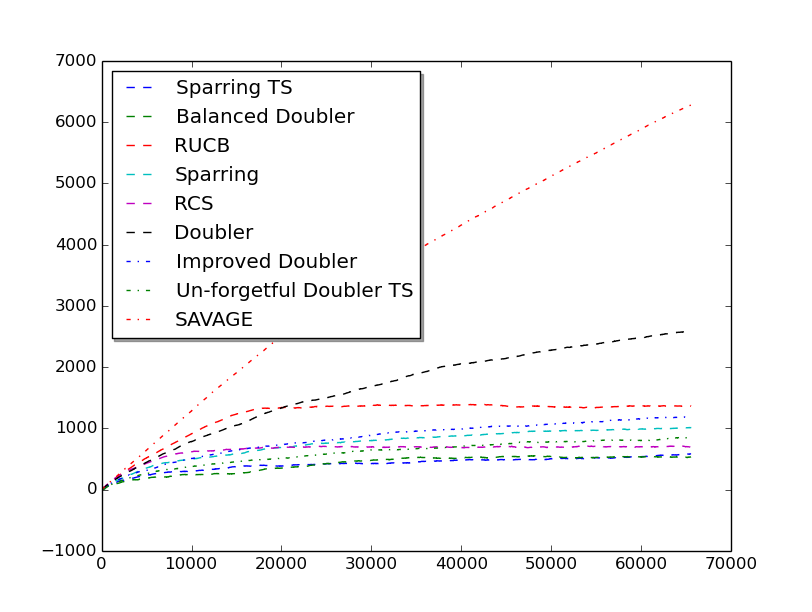
\includegraphics[scale=0.5]{figures/all_MQ2007_7arms.png}
  \caption{Utility Based Regret with 7 Arms}
\end{figure}

For a larger number of arms we can see that RCS and RUCB are outperformed by the other algorithms.

\begin{figure}[h!]
\centering
  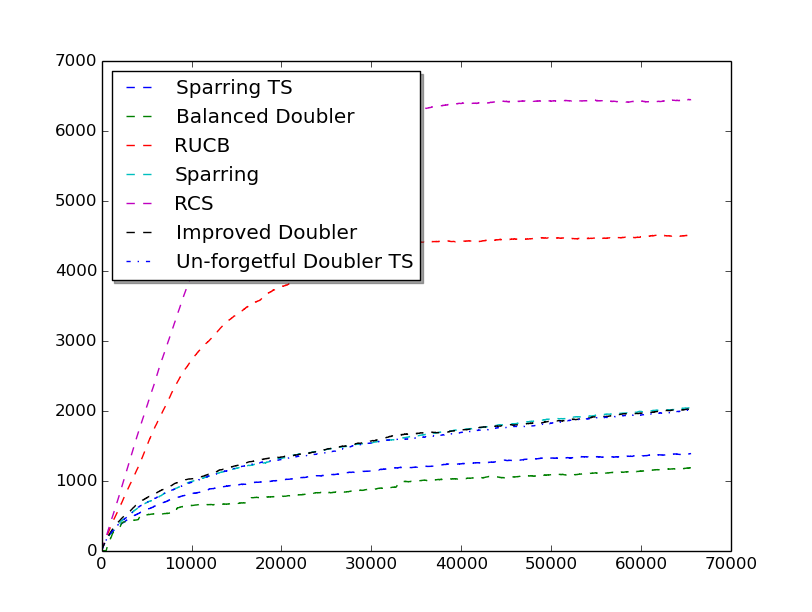
\includegraphics[scale=0.5]{figures/all_MQ2007_24arms.png}
  \caption{Utility Based Regret with 24 Arms}
\end{figure}

And for 46 arms we can see that Sparring with Thompson Sampling methods performs better than all the other algorithms.


\subsection{Sparring}

We can see the clear advantage of using the Sparring algorithm over the RCS algorithm when dealing with a large number of arms.
\begin{figure}[h!]
\centering
\begin{subfigure}{.5\textwidth}
  \centering
  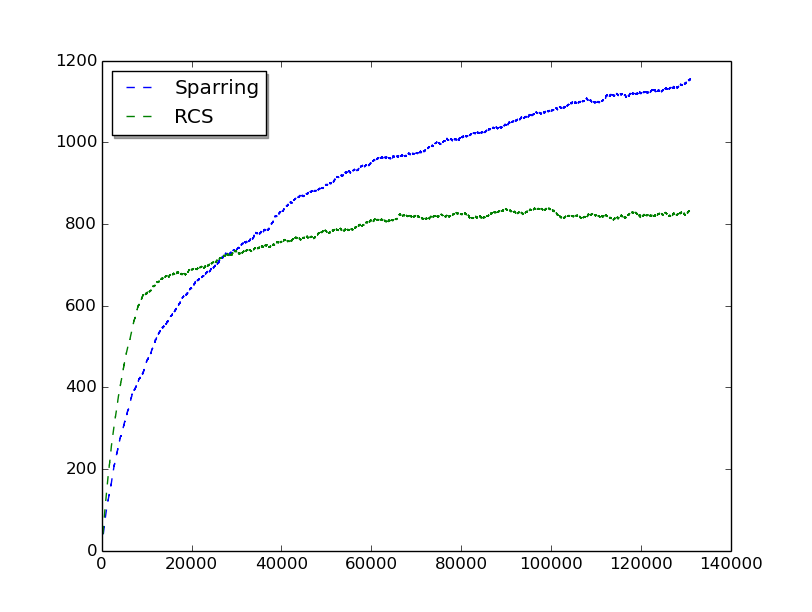
\includegraphics[scale=0.3]{figures/rcs_sparring_MQ2007_7arms.png}
  \caption{7 Arms}
  \label{fig:sub1}
\end{subfigure}%
\begin{subfigure}{.5\textwidth}
  \centering
  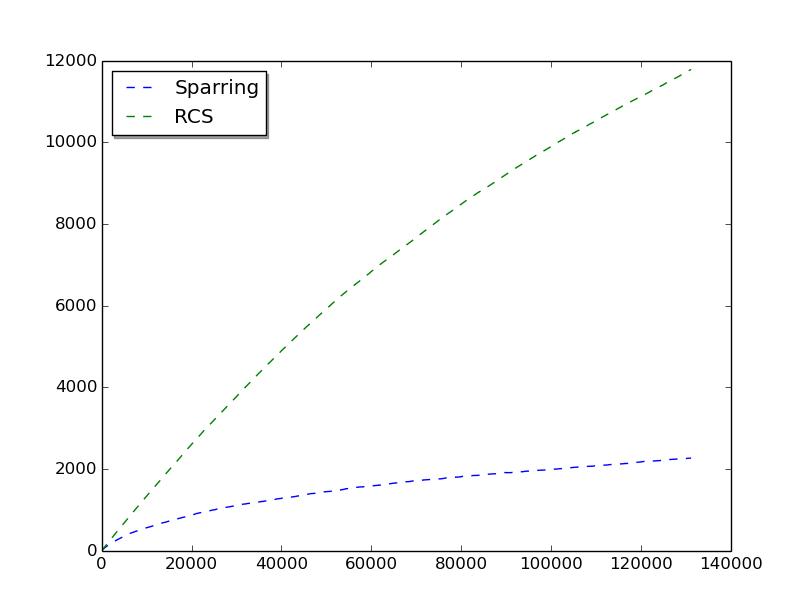
\includegraphics[scale=0.3]{figures/rcs_sparring_MQ2007_16arms.png}
  \caption{16 Arms}
  \label{fig:sub2}
\end{subfigure}
\begin{subfigure}{.5\textwidth}
  \centering
  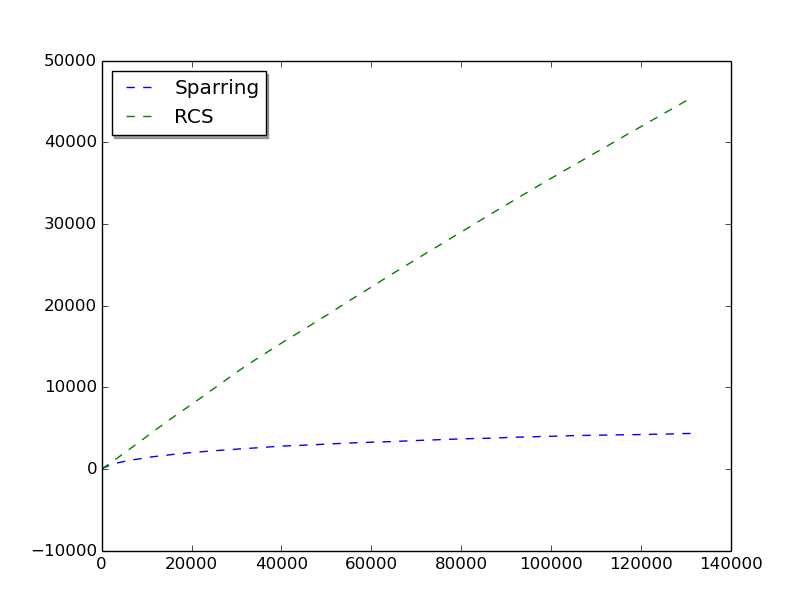
\includegraphics[scale=0.3]{figures/rcs_sparring_MQ2007_46arms.png}
  \caption{46 Arms}
  \label{fig:sub2}
\end{subfigure}
\caption{RCS Versus Sparring with Utility Based Regret}
\label{fig:test}
\end{figure}


With a small number of arms (Fig 1.) we can observe that the RCS algorithm quickly converges to the optimal arm.
\\
With a larger number of arms we can see that Sparring out-performs the RCS algorithm. 
\\
Now lets look at the general regret (as defined section 2.2). Here we used 46 arms:
\begin{figure}[h!]
  \centering
     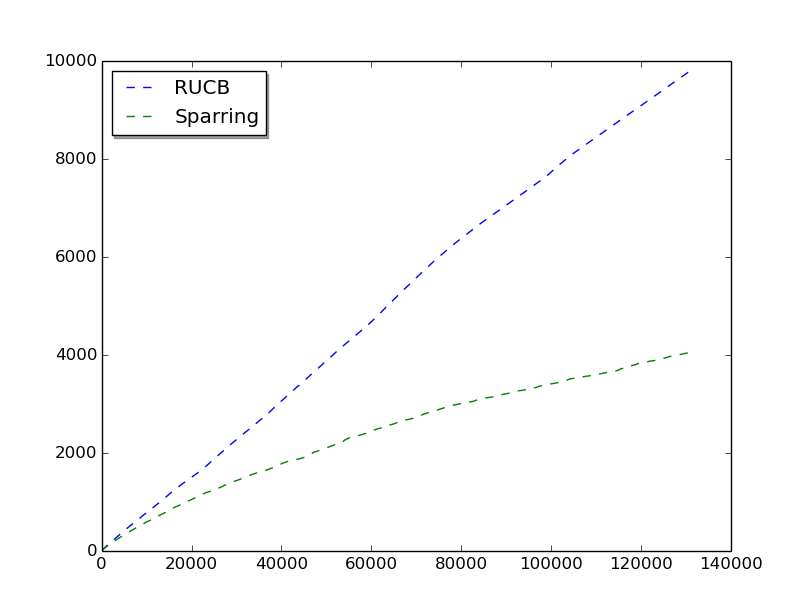
\includegraphics[scale=0.4]{figures/rcs_sparring_MQ2007_general.png} 
  \caption{RCS Versus Sparring with Preference Based Regret with 46 Arms}
\end{figure}


\newpage
\subsection{Doubler}
Now lets have a look at the Doubler algorithm using the same data set.
\begin{figure}[h!]
\centering
\begin{subfigure}{.5\textwidth}
  \centering
  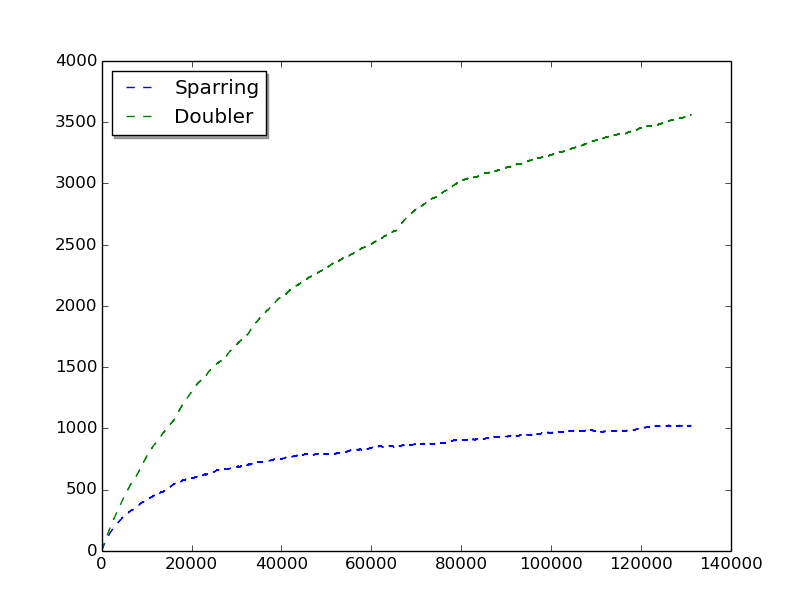
\includegraphics[scale=0.3]{figures/doubler_sparring_MQ2007_7arms.png}
  \caption{7 Arms}
  \label{fig:sub1}
\end{subfigure}%
\begin{subfigure}{.5\textwidth}
  \centering
  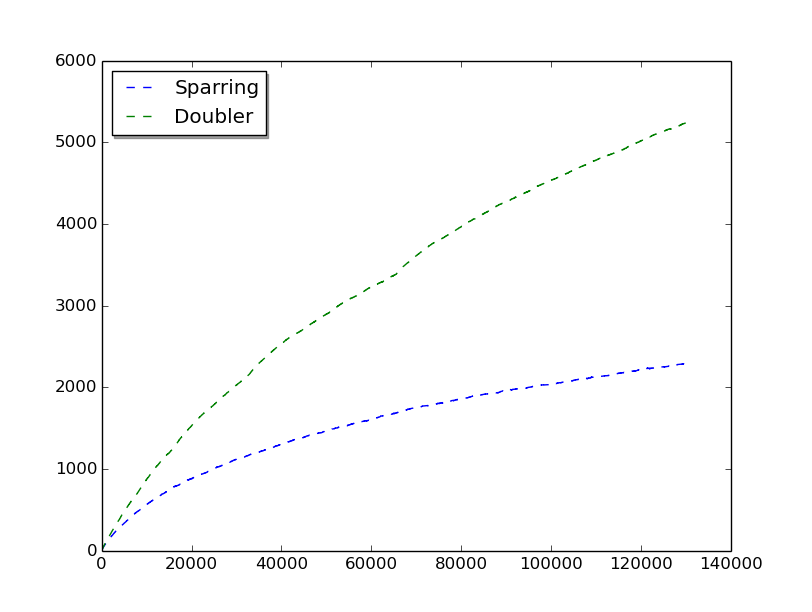
\includegraphics[scale=0.3]{figures/doubler_sparring_MQ2007_16arms.png}
  \caption{16 Arms}
  \label{fig:sub2}
\end{subfigure}
\begin{subfigure}{.5\textwidth}
  \centering
  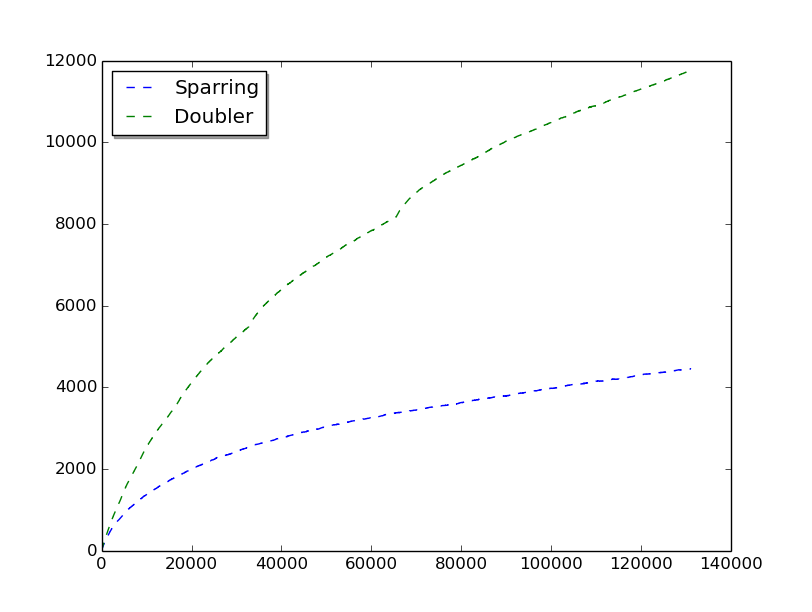
\includegraphics[scale=0.3]{figures/doubler_sparring_MQ2007_46arms.png}
  \caption{46 Arms}
  \label{fig:sub2}
\end{subfigure}
\caption{Doubler Versus Sparring with Utility Based Regret}
\label{fig:test}
\end{figure}

The general regret:
\begin{figure}[h!]
  \centering
     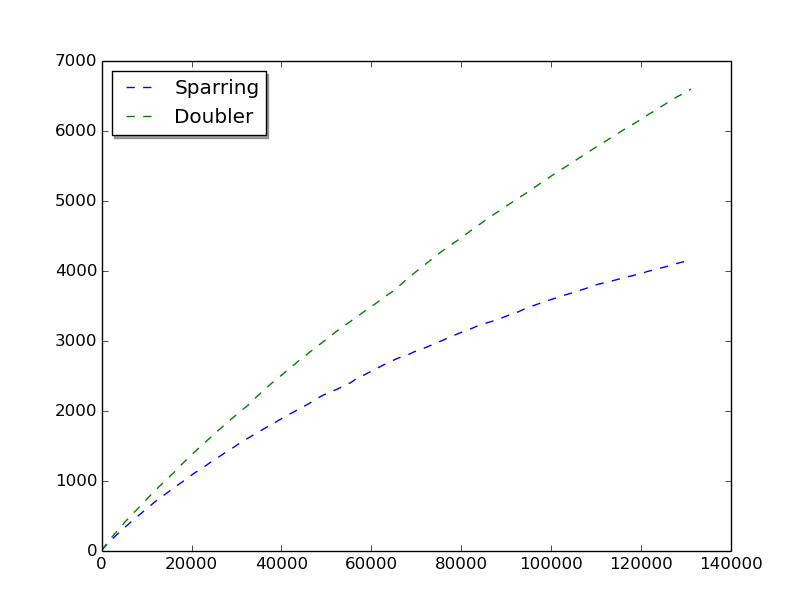
\includegraphics[scale=0.2]{figures/doubler_sparring_MQ2007_general.png} 
  \caption{Doubler Versus Sparring with Preference Based Regret with 46 Arms}
\end{figure}

\newpage
\subsection{Improved Doubler}
Now lets have a look at the Improved Doubler algorithm using the same data set.
\begin{figure}[h!]
\centering
\begin{subfigure}{.5\textwidth}
  \centering
  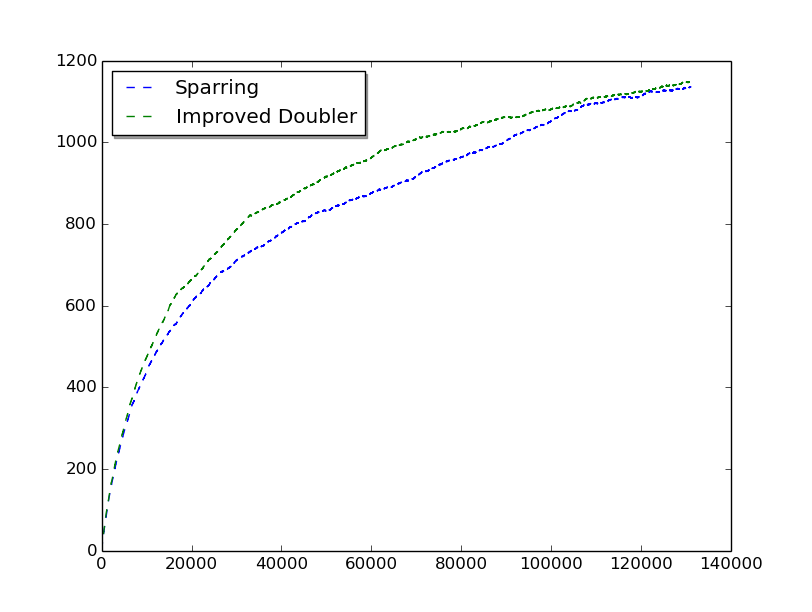
\includegraphics[scale=0.3]{figures/improved_doubler_sparring_MQ2007_7arms.png}
  \caption{7 Arms}
  \label{fig:sub1}
\end{subfigure}%
\begin{subfigure}{.5\textwidth}
  \centering
  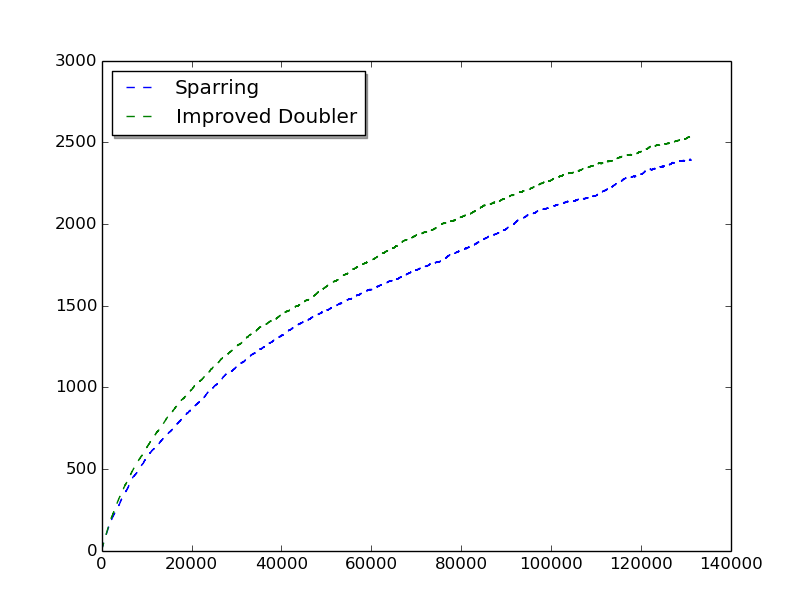
\includegraphics[scale=0.3]{figures/improved_doubler_sparring_MQ2007_16arms.png}
  \caption{16 Arms}
  \label{fig:sub2}
\end{subfigure}
\begin{subfigure}{.5\textwidth}
  \centering
  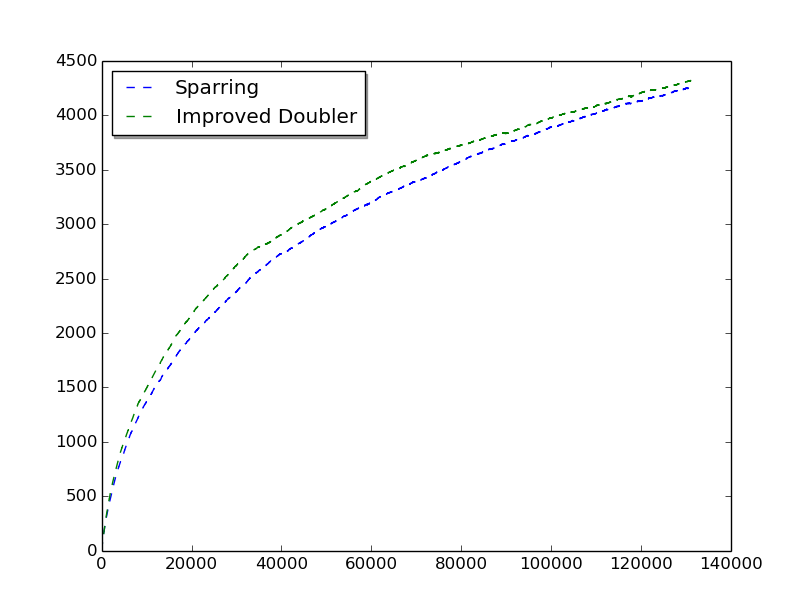
\includegraphics[scale=0.3]{figures/improved_doubler_sparring_MQ2007_46arms.png}
  \caption{46 Arms}
  \label{fig:sub2}
\end{subfigure}
\caption{Improved Doubler Versus Sparring with Utility Based Regret}
\label{fig:test}
\end{figure}

The general regret:
\begin{figure}[h!]
  \centering
     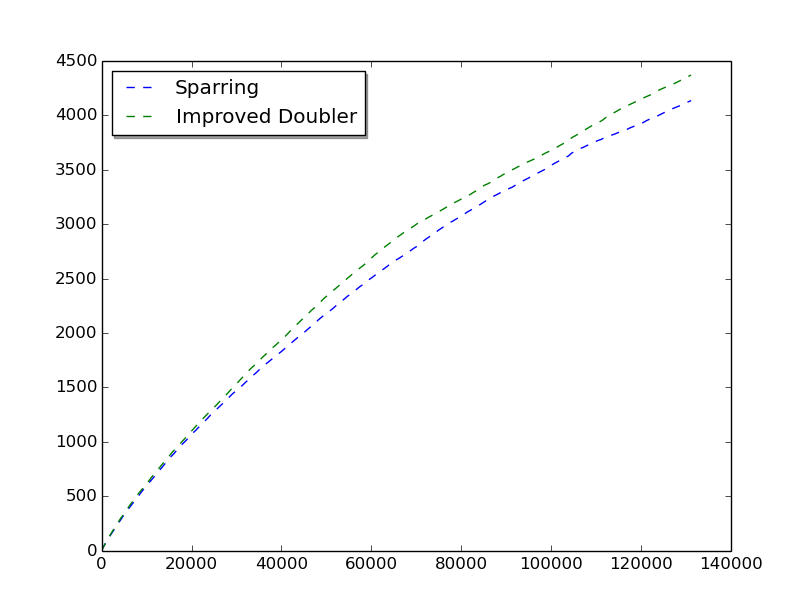
\includegraphics[scale=0.3]{figures/improved_doubler_sparring_MQ2007_general.png} 
  \caption{Improved Doubler Versus Sparring with Preference Based Regret with 46 Arms}
\end{figure}
\newpage
\subsection{Balanced Doubler}
Now lets have a look at the Balanced Doubler algorithm using the same data set.
\begin{figure}[h!]
  \centering
     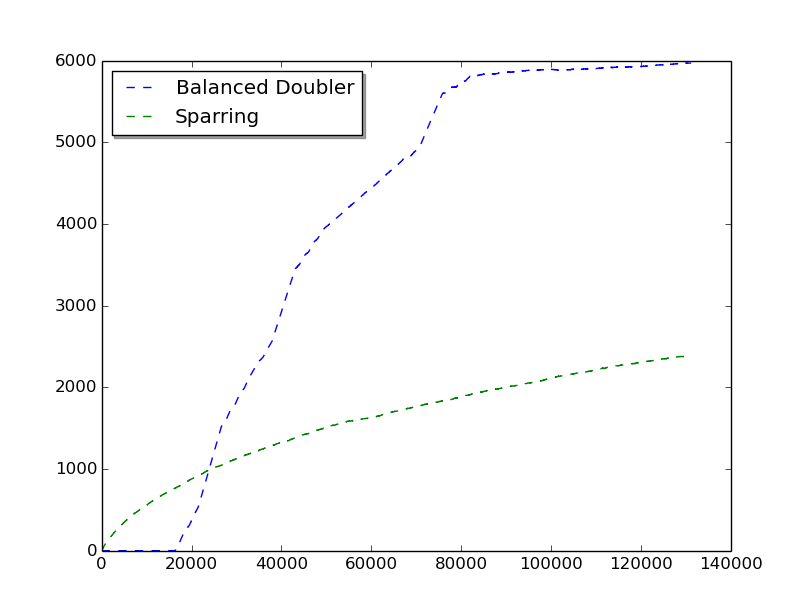
\includegraphics[scale=0.3]{figures/balanced_doubler_sparring_MQ2007_16arms.png} 
  \caption{Balanced Doubler Versus Sparring with Utility Based Regret with 16 Arms}
\end{figure}

\subsection{Thompson Sampling Doubler}
Now lets have a look at the Balanced Doubler algorithm using the same data set.
\begin{figure}[h!]
\centering
\begin{subfigure}{.5\textwidth}
  \centering
  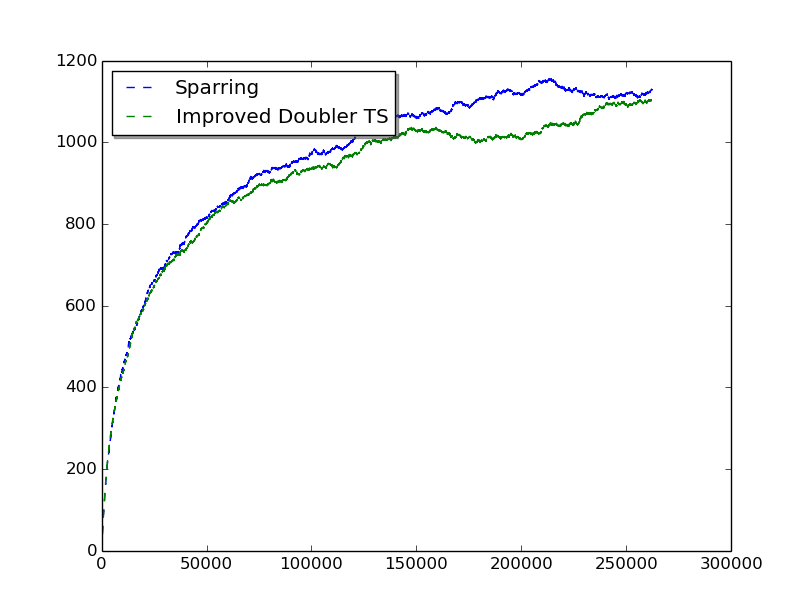
\includegraphics[scale=0.3]{figures/improved_doubler_TS_sparring_MQ2007_7arms.png}
  \caption{7 Arms}
  \label{fig:sub1}
\end{subfigure}%
\begin{subfigure}{.5\textwidth}
  \centering
  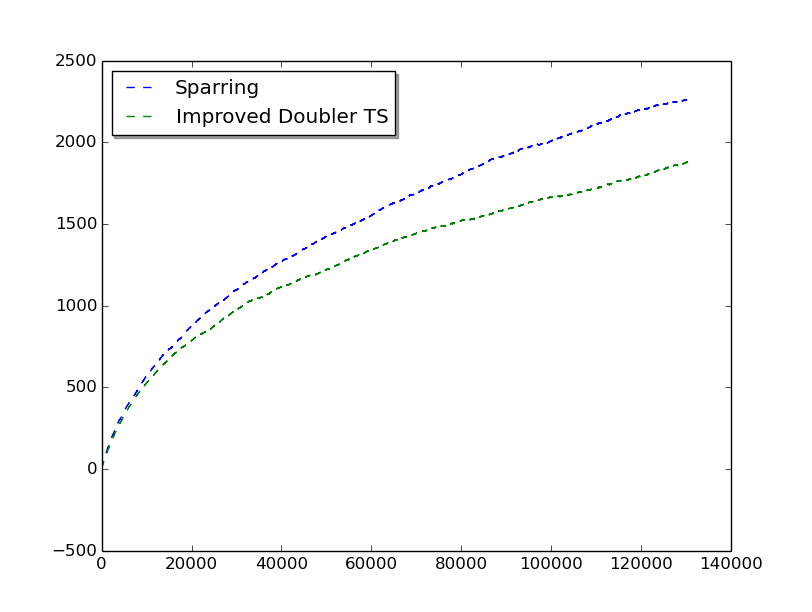
\includegraphics[scale=0.3]{figures/improved_doubler_TS_sparring_MQ2007_16arms.png}
  \caption{16 Arms}
  \label{fig:sub2}
\end{subfigure}
\begin{subfigure}{.5\textwidth}
  \centering
  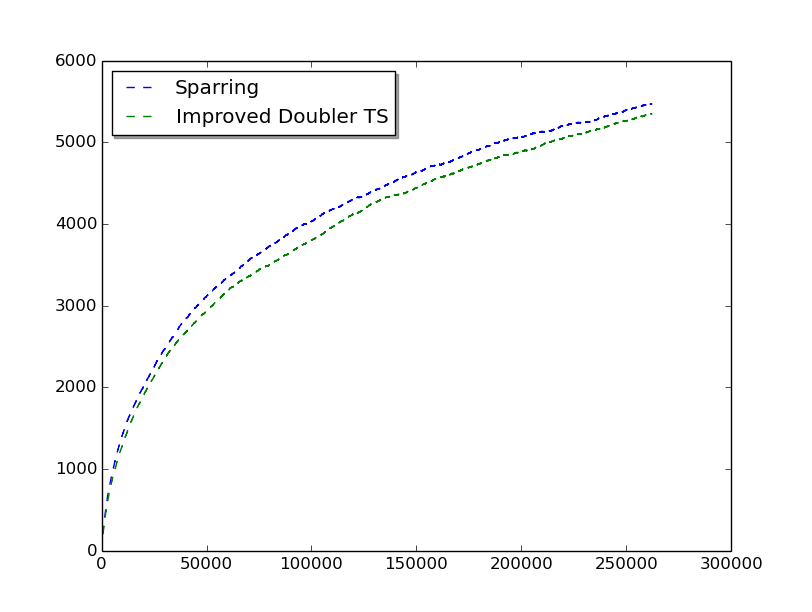
\includegraphics[scale=0.3]{figures/improved_doubler_TS_sparring_MQ2007_46arms.png}
  \caption{46 Arms}
  \label{fig:sub2}
\end{subfigure}
\caption{Improved Doubler Versus Sparring with Utility Based Regret}
\label{fig:test}
\end{figure}

The general regret:
\begin{figure}[h!]
  \centering
     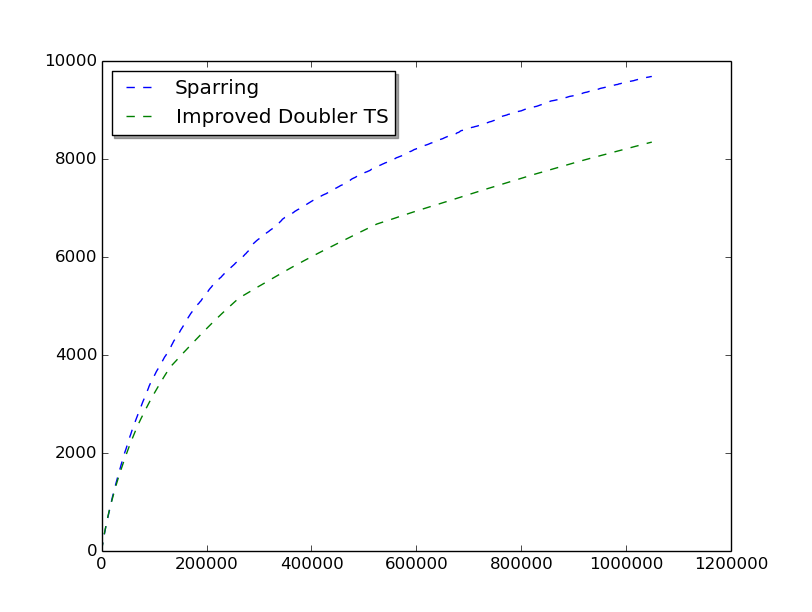
\includegraphics[scale=0.4]{figures/improved_doubler_TS_sparring_MQ2007_general.png} 
  \caption{Improved Doubler Versus Sparring with Preference Based Regret with 46 Arms}
\end{figure}

\subsection{Thompson Sampling Sparring}
And finally, lets show the results of  the sparring algorithm when using Thompson Sampling black boxes.

\begin{figure}[h!]
  \centering
     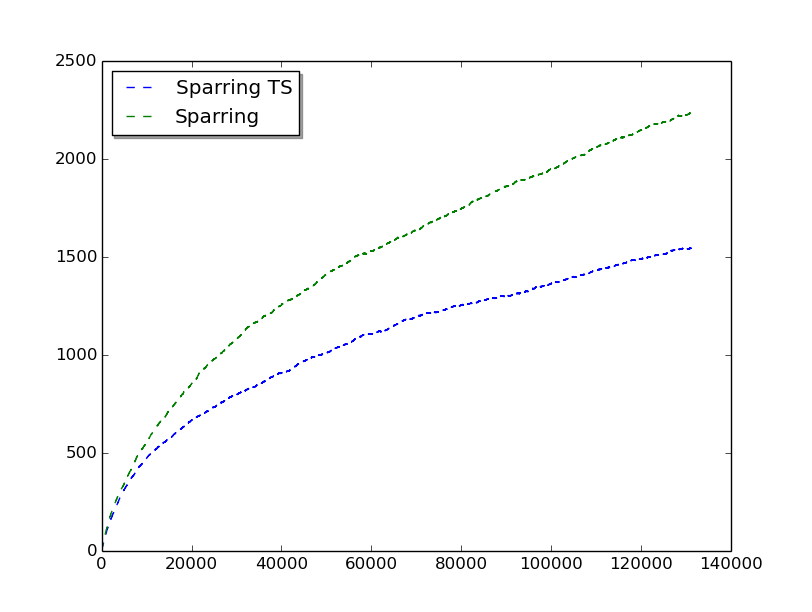
\includegraphics[scale=0.4]{figures/TS_sparring_sparring_MQ2007_16arms.png} 
  \caption{Thompson Sampling Sparring Versus Sparring with Utility Based Regret with 16 Arms}
\end{figure}

The general regret:
\begin{figure}[h!]
  \centering
     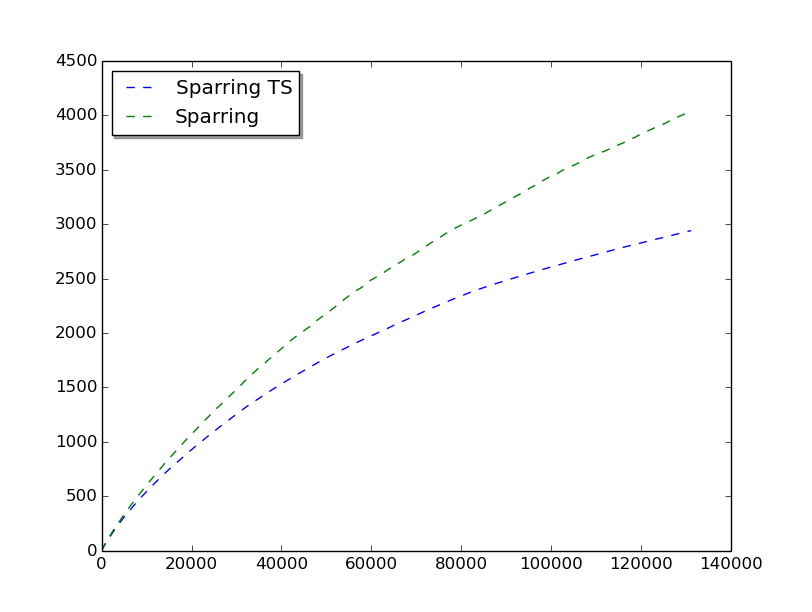
\includegraphics[scale=0.4]{figures/TS_sparring_sparring_MQ2007_general.png} 
  \caption{Thompson Sampling Sparring Versus Sparring with Preference Based Regret with 46 Arms}
\end{figure}

\end{document}
